\documentclass[10pt]{article}
\usepackage[margin=0.72in]{geometry}
\usepackage[T1]{fontenc}
\usepackage{lmodern}
\usepackage{graphicx}
\usepackage{booktabs}
\usepackage{microtype}
\usepackage{xcolor}
\usepackage{hyperref}
\hypersetup{colorlinks=true,linkcolor=blue,urlcolor=blue}
\setlength{\parskip}{5pt}
\setlength{\parindent}{0pt}
\newcommand{\code}[1]{\texttt{\small #1}}
\begin{document}

{\Large\bfseries EXP-ECDLP-6dacdb execution report}\par
\emph{Observation-only record for \code{RUN-ECDLP-36b2a5} and \code{RUN-ECDLP-994eb9}.}

This report records the completed process, checker outputs, and measured
quantities; it does not assign evidence strength, change the hypothesis or
experiment state, or make a scientific verdict.

\begin{center}
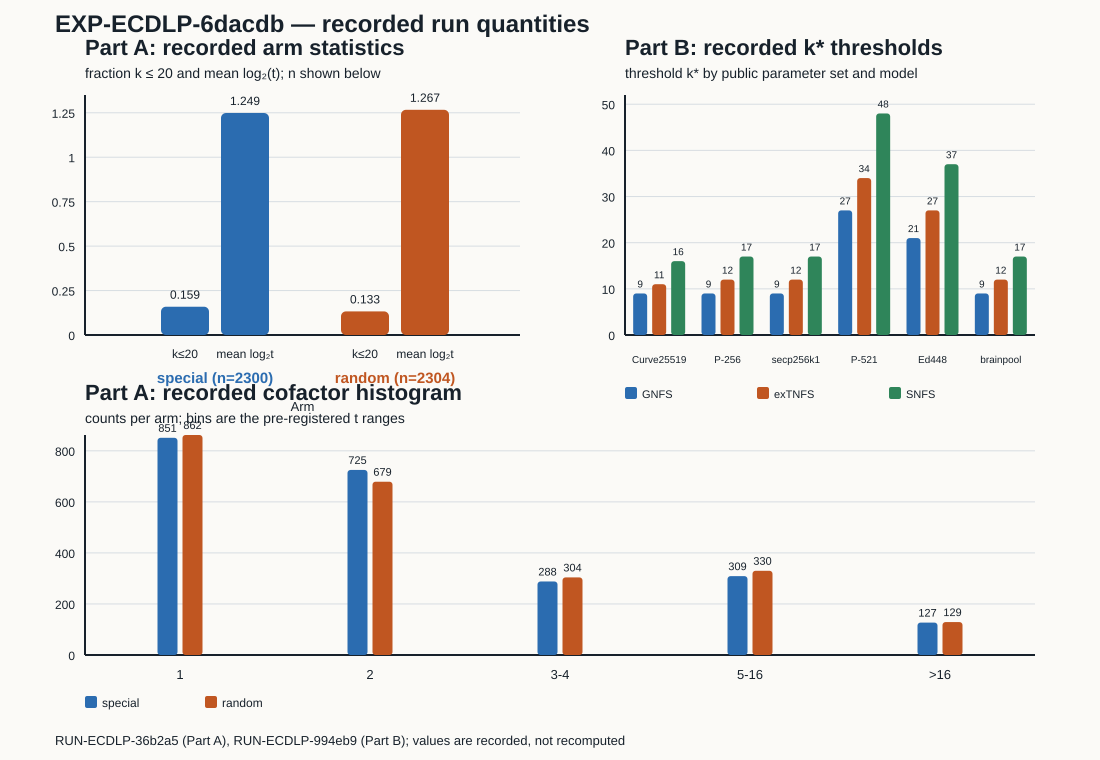
\includegraphics[width=\textwidth]{graph.svg}
\end{center}

\section*{Scope and custody}
\begin{itemize}
\item Goal \code{GOAL-ECDLP-001}; question \code{RQ-ECDLP-002}; hypothesis
\code{H-ECDLP-bd1572}; experiment \code{EXP-ECDLP-6dacdb}.
\item Corrected frozen plan \code{experiments/EXP-ECDLP-6dacdb/trial-plan-v2.json},
SHA-256 \code{798321ec3932d92a09eede9152fe198d72d2aeab6e7e9d6502fafc3790fa0567}.
The additive dispatch correction is \code{CORR-20261011-2c3e1f}; it changes
queue binding and task/run identifiers, not scientific fields or source hashes.
\item Queue \code{BATCH-62ac7b}; executor \code{TASK-20261011-672eaf}; owner
\code{executor-ecdlp-6dacdb-v2}, epoch 1. The receipts record dispatch-plan
SHA-256 \code{b7940519fd5c0c4068dda9f7f3dbbe030e5598b53ac9ae0c073a7f78c6d4c614}.
\item Remote execution commit \code{2f5957be13584d31dd0b2ace1815a1d3aec7e6fa};
Linux; Python 3.12.11. The specification SHA-256 is
\code{2649c4cabb8f97626f9e6406abf80ae51d26fe7b0fa4a882b7d3ac25c751a185}.
The sealed environments record the source hashes for \code{check.py},
\code{primeset.py}, and \code{run.py}; their full values are in the Markdown
report and both run directories.
\item The local archival worktree had unrelated untracked artifacts during
import. Hostname and CPU-time measurements were not present in the sealed
environment or manifest and are missing rather than inferred. Run-record
commit \code{ea813bd52a} was pushed before this report was created.
\end{itemize}

\section*{Trials and process results}
Two trials were requested and two completed. Both receipts have
\code{status: output\_validated}, \code{returncode: 0},
\code{check\_returncode: 0}, and no recorded scientific conclusion. The
independent checker returned zero errors for each sealed run.

\textbf{Part A.} \code{RUN-ECDLP-36b2a5} ran from
\code{2026-10-11T20:35:23.712268Z} to
\code{2026-10-11T20:35:59.065855Z}; recorded wall time was
\code{34.765450954437256 s}. The command was
\code{python3 ... run.py --part A --seeds 1 2 3 --curves 64 --out <run\_dir>}.
The raw result has 72 cells and records 2,300 special-arm and 2,304 random-arm
non-anomalous samples. The checker log reports 12 curve rows recounted and zero
errors.

\textbf{Part B.} \code{RUN-ECDLP-994eb9} ran from
\code{2026-10-11T20:35:59.150197Z} to
\code{2026-10-11T20:36:00.910884Z}; recorded wall time was
\code{1.7606866359710693 s}. The command was
\code{python3 ... run.py --part B --out <run\_dir>}.
The six declared public parameter sets were processed, with order search bound
\code{10^6}; the checker log reports zero curve-row errors.

\section*{Recorded observations}
The graph plots values directly from the raw results; \code{plot\_data.json} is
the extracted plotting data and \code{plot.py} is the SVG renderer.

\textbf{Part A.} The recorded \code{k <= 20} fractions were 0.1591304348
(special, \code{n=2300}) and 0.1328125 (random, \code{n=2304}). The recorded
difference was 0.0263179348 with standard error 0.0104002785. Mean
\code{log2(t)} was 1.2486514049 and 1.2667237009, with difference
-0.0180722961 and recorded permutation p-value 0.6835316468. The histogram
counts in bins \code{1}, \code{2}, \code{3--4}, \code{5--16}, and \code{>16}
were [851,725,288,309,127] and [862,679,304,330,129]. The recorded
chi-square was 2.7124839037 with permutation p-value 0.6116941529. The 43
nearby supersingular controls all recorded \code{k=2}; the checker returned
zero errors.

\textbf{Part B.} All six rows recorded the first searched embedding degree as
\code{> 1,000,000}. The displayed \code{k*} table is:

\begin{center}
\begin{tabular}{lrrrr}
\toprule
Parameter set & GNFS & exTNFS & SNFS/STNFS & $\log_2$ rho\\
\midrule
Curve25519 & 9 & 11 & 16 & 125.8254\\
P-256 & 9 & 12 & 17 & 127.8254\\
secp256k1 & 9 & 12 & 17 & 127.8254\\
P-521 & 27 & 34 & 48 & 260.3254\\
Ed448 & 21 & 27 & 37 & 222.8254\\
brainpoolP256r1 & 9 & 12 & 17 & 127.5300\\
\bottomrule
\end{tabular}
\end{center}

The source table labels the constants recalled and optimistic and drops the
$o(1)$ term. All six rows record prime checks and Hasse checks true. Five rows
record a bound-point order check true; Ed448 is \code{null} because no base
point was bound in this invocation and its order is marked recalled-only.

As derived arithmetic only, the largest displayed threshold is 48; combined
with the recorded lower bound this gives a lower-bound difference greater than
999,952 in $k$ units. This is not an additional measurement.

\section*{Missing data and boundary}
CPU time, machine hostname, and runtime lock hash were not recorded. No extra
samples, curves, constants, or secret-dependent computation were run. The
graph and report cover only these two completed trials and their declared
scopes. Raw results, manifests, receipts, commands, environments, checker
logs, and the Part B table remain in the two run directories. Scientific
interpretation and any official state transition remain for independent
review/archive tasks.

\end{document}
